%%%%%%%%%%%%%%%%%%%%%%%%%%%%%%%%%%%%%%%%%%%%%%%%%%%%%%%%%%%%%%
% School Management System - Final Year Diploma Project Report
% LaTeX Template (for Overleaf or other compilers)
%%%%%%%%%%%%%%%%%%%%%%%%%%%%%%%%%%%%%%%%%%%%%%%%%%%%%%%%%%%%%%
\documentclass[12pt,a4paper]{report}
\usepackage[utf8]{inputenc}
\usepackage{graphicx}
\usepackage[a4paper, left=1.5in, right=1in, top=1in, bottom=1in]{geometry}
\usepackage{array}
\usepackage{enumitem}
\usepackage{titlesec}
\usepackage{amsmath}
\usepackage{amsfonts}
\usepackage{amssymb}
\usepackage{mathptmx} % Better Times New Roman implementation
\usepackage[T1]{fontenc} % Better font encoding
\usepackage{url} % For hyperlinking URLs
\usepackage{fancyhdr}
\usepackage{setspace}
\usepackage{hyperref}
\usepackage{longtable}
\usepackage{tocloft}
\usepackage{caption}
\usepackage{booktabs}

% Page Setup
\setstretch{1.5}
\pagestyle{fancy}
\fancyhf{}
\fancyfoot[C]{\thepage}

% Customizing section titles to match the document's style (simple and bold)
\titleformat{\chapter}[hang]{\bfseries\LARGE}{\thechapter}{2em}{}
\titleformat{\section}[hang]{\bfseries\large}{\thesection}{1em}{}
\titleformat{\subsection}[hang]{\bfseries}{\thesubsection}{1em}{}
\titleformat{\subsubsection}
  {\normalfont\normalsize\bfseries}{\thesubsubsection}{1em}{}

% Remove page number on the first page (cover page)
\pagenumbering{gobble}

\begin{document}

% --- Cover Page ---
\begin{titlepage}
    \centering
    \vspace*{0.3cm}
    
    
\includegraphics[width=3.5cm]{nibm-logo.png} % NIBM Logo
    
    \vspace{1cm}
    
    {\Huge\bfseries NATIONAL INSTITUTE OF BUSINESS MANAGEMENT}
    
    \vspace{1cm}
    
    {\Large School of Computing and Engineering}
    
    \vspace{1.2cm}
    
    {\Huge\bfseries ``School Management System''}
    
    \vspace{1.2cm}
    
    {\Large\bfseries Final Year Diploma Project Report}
    
    {\large Academic Year 2022-23}
    
    \vspace{1.5cm}
    
    {\Large Submitted By:}
    
    \vspace{0.5cm}
    
    {\large E M A S B EKANAYAKA (CODSE224F-001)}
    
    {\large S D HEIYANTHUDUWA (CODSE224F-016)}
    
    {\large M H D T TISSERA (CODSE224F-054)}
    
    \vspace{1cm}
    
    {\Large Project Guide:}
    
    \vspace{0.3cm}
    
    {\Large\bfseries DR. THISARA WEERASINGHE}
    
    {\large Head of School of Computing and Engineering}
    
    \vfill % Pushes content to the bottom
    
    {\large Date: 2024/12/20}
    
    {\large Place: NIBM Colombo School of Computing and Engineering}
    
    \vspace{0.5cm}
    
    {\Large\bfseries Diploma in Software Engineering}
    
\end{titlepage}

\newpage
\pagenumbering{roman} % Start page numbering from here with Roman numerals

% --- Coursework Content ---

%%%%%%%%%%%%%%%%%%%%%%%%%%%%%%%%%%%%%%%%%%%%%%%%%%%%%%%%%%%%%%
% Declaration Page
%%%%%%%%%%%%%%%%%%%%%%%%%%%%%%%%%%%%%%%%%%%%%%%%%%%%%%%%%%%%%%
\section*{Declaration}
I/We hereby declare that this project report is my/our own work and has not been submitted previously for any academic qualification. All sources of information have been acknowledged.

\vspace{2cm}
\noindent\textbf{Signatures:}

\vspace{2cm}
\noindent\rule{6cm}{0.4pt}\\
\noindent E M A S B EKANAYAKA (CODSE224F-001)

\vspace{1cm}
\noindent\rule{6cm}{0.4pt}\\
\noindent S D HEIYANTHUDUWA (CODSE224F-016)

\vspace{1cm}
\noindent\rule{6cm}{0.4pt}\\
\noindent M H D T TISSERA (CODSE224F-054)

%%%%%%%%%%%%%%%%%%%%%%%%%%%%%%%%%%%%%%%%%%%%%%%%%%%%%%%%%%%%%%
% Abstract
%%%%%%%%%%%%%%%%%%%%%%%%%%%%%%%%%%%%%%%%%%%%%%%%%%%%%%%%%%%%%%
\newpage
\section*{Abstract}
The School Management System is a comprehensive software solution designed to address the growing needs of modern educational institutions. This project implements a robust platform that integrates various aspects of school administration, academic management, and communication into a unified system. The system employs cutting-edge technologies including biometric authentication, role-based access control, and real-time data processing to provide an efficient and secure environment for all stakeholders.

The implementation demonstrates significant improvements in administrative efficiency, reducing manual workload through automation of routine tasks and streamlining communication channels, thereby enhancing the overall educational experience. The system's modular architecture ensures scalability and maintainability, while its intuitive interface promotes rapid adoption among users of varying technical proficiency.

The project's significance lies in its potential to transform traditional educational management practices, particularly in government schools where resources are often limited. By digitizing core processes and providing real-time access to information, the system enables better decision-making and more effective resource utilization, ultimately contributing to improved educational outcomes.

\textbf{Keywords:} School Management, Education Technology, Academic Administration, Database Management, Web Application

%%%%%%%%%%%%%%%%%%%%%%%%%%%%%%%%%%%%%%%%%%%%%%%%%%%%%%%%%%%%%%
% List of Keywords, Figures, Tables, Acronyms, Acknowledgement
%%%%%%%%%%%%%%%%%%%%%%%%%%%%%%%%%%%%%%%%%%%%%%%%%%%%%%%%%%%%%%
\newpage
\section*{Acknowledgement}
We would like to express our sincere gratitude to our project guide, Dr. Thisara Weerasinghe, and the faculty of the School of Computing and Engineering for their invaluable support and guidance throughout this project.

%%%%%%%%%%%%%%%%%%%%%%%%%%%%%%%%%%%%%%%%%%%%%%%%%%%%%%%%%%%%%%
% Table of Contents
%%%%%%%%%%%%%%%%%%%%%%%%%%%%%%%%%%%%%%%%%%%%%%%%%%%%%%%%%%%%%%
\newpage
\tableofcontents

%%%%%%%%%%%%%%%%%%%%%%%%%%%%%%%%%%%%%%%%%%%%%%%%%%%%%%%%%%%%%%
% List of Figures and Tables
%%%%%%%%%%%%%%%%%%%%%%%%%%%%%%%%%%%%%%%%%%%%%%%%%%%%%%%%%%%%%%
\newpage
\listoffigures

\newpage
\listoftables

\newpage
\renewcommand{\thepage}{\arabic{page}} % Switch to Arabic numerals
\setcounter{page}{1}

%%%%%%%%%%%%%%%%%%%%%%%%%%%%%%%%%%%%%%%%%%%%%%%%%%%%%%%%%%%%%%
% Chapter 1: Introduction
%%%%%%%%%%%%%%%%%%%%%%%%%%%%%%%%%%%%%%%%%%%%%%%%%%%%%%%%%%%%%%
\chapter{Introduction}
\section{Background}
The digital revolution has transformed virtually every sector of society, yet many educational institutions, particularly government schools, continue to operate using traditional manual systems. This technological gap not only impacts administrative efficiency but also affects the quality of education and student engagement. In an era where students are increasingly tech-savvy and parents expect real-time updates about their children's progress, the need for a comprehensive digital solution has become paramount.

\section{Project Context}
This School Management System project emerges from a critical need to modernize educational institution operations in government schools. The initiative was conceived after extensive consultation with educators, administrators, and education technology experts, who identified significant opportunities for improving educational outcomes through digital transformation.

\section{Project Objectives}
\begin{itemize}
    \item Modernization of Educational Operations
    \item Improvement of Stakeholder Engagement
\end{itemize}

\section{Scope and Significance}
The project encompasses a complete overhaul of school management processes, from daily administrative tasks to long-term strategic planning. Its significance lies in its potential to:
\begin{itemize}
    \item Reduce administrative burden through automation
    \item Enhance student performance tracking accuracy with digital records
\end{itemize}

%%%%%%%%%%%%%%%%%%%%%%%%%%%%%%%%%%%%%%%%%%%%%%%%%%%%%%%%%%%%%%
% Chapter 2: Methodology
%%%%%%%%%%%%%%%%%%%%%%%%%%%%%%%%%%%%%%%%%%%%%%%%%%%%%%%%%%%%%%
\chapter{Methodology}
\section{Introduction}
The methodology adopted for this project follows a structured software development lifecycle, including requirements gathering, system analysis, design, implementation, and testing. Data collection techniques included interviews, questionnaires, and document reviews with stakeholders.

\section{Development Approach}
A phased development approach was used:
\begin{itemize}
    \item \textbf{Phase 1: Foundation} -- User authentication, profile management, database setup
    \item \textbf{Phase 2: Core Functionality} -- Academic management, attendance tracking, and assessment features
    \item \textbf{Phase 3: Advanced Features} -- Reporting, communication platform, analytics dashboard
\end{itemize}

\section{Chapter Summary}
This chapter outlined the methodology and development approach used to ensure the system meets stakeholder requirements and is delivered on time.

%%%%%%%%%%%%%%%%%%%%%%%%%%%%%%%%%%%%%%%%%%%%%%%%%%%%%%%%%%%%%%
% Chapter 3: Analysis
%%%%%%%%%%%%%%%%%%%%%%%%%%%%%%%%%%%%%%%%%%%%%%%%%%%%%%%%%%%%%%
\chapter{Analysis}
\section{Current Environment Assessment}
Government schools often operate with limited resources and manual processes, leading to inefficiencies and data management challenges. The current environment was assessed through stakeholder interviews and process mapping.

\section{Feasibility Study}
A feasibility study was conducted to evaluate technical, operational, and economic viability. The results indicated strong potential for improvement through digital transformation.

\section{Problem Statement}
Teachers spend considerable time on administrative tasks that could be automated, while parents struggle to stay informed about their children's progress. The lack of standardized processes and difficulty in tracking student performance data are key issues.

\section{Chapter Summary}
This chapter analyzed the current system, identified limitations, and established the need for a comprehensive school management solution.

%%%%%%%%%%%%%%%%%%%%%%%%%%%%%%%%%%%%%%%%%%%%%%%%%%%%%%%%%%%%%%
% Chapter 4: Solution Design
%%%%%%%%%%%%%%%%%%%%%%%%%%%%%%%%%%%%%%%%%%%%%%%%%%%%%%%%%%%%%%
\chapter{Solution Design}
\section{System Architecture}
The system is designed with a modular architecture, ensuring scalability and maintainability. Key modules include authentication, academic management, attendance, assessment, reporting, and communication.

\begin{table}[htbp]
    \centering
    \caption{Technologies Used}
    \label{tab:tech-stack}
    \begin{tabular}{ll}
        \toprule
        Category & Technology \\
        \midrule
        Frontend & HTML, CSS, JavaScript \\
        Backend & Node.js, Express.js \\
        Database & MySQL \\
        Version Control & Git \\
        \bottomrule
    \end{tabular}
\end{table}

\section{Design Patterns and Principles}
The design follows best practices such as separation of concerns, robust error handling, and secure data flow. Standardized API interfaces and middleware facilitate integration between modules.

\section{System Modeling and Documentation}
\subsection{Entity-Relationship Diagram}
\begin{figure}[htbp]
    \centering
    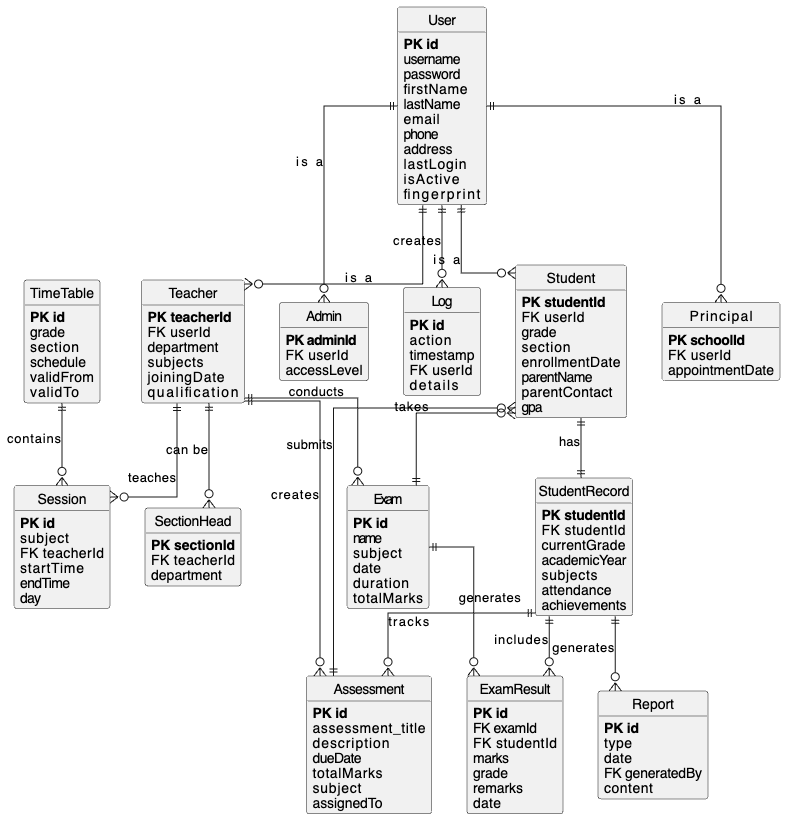
\includegraphics[width=1\textwidth]{er-diagram.png}
    \caption{Entity-Relationship Diagram}
    \label{fig:er-diagram}
\end{figure}

\subsection{Class Diagram}
\begin{figure}[htbp]
    \centering
    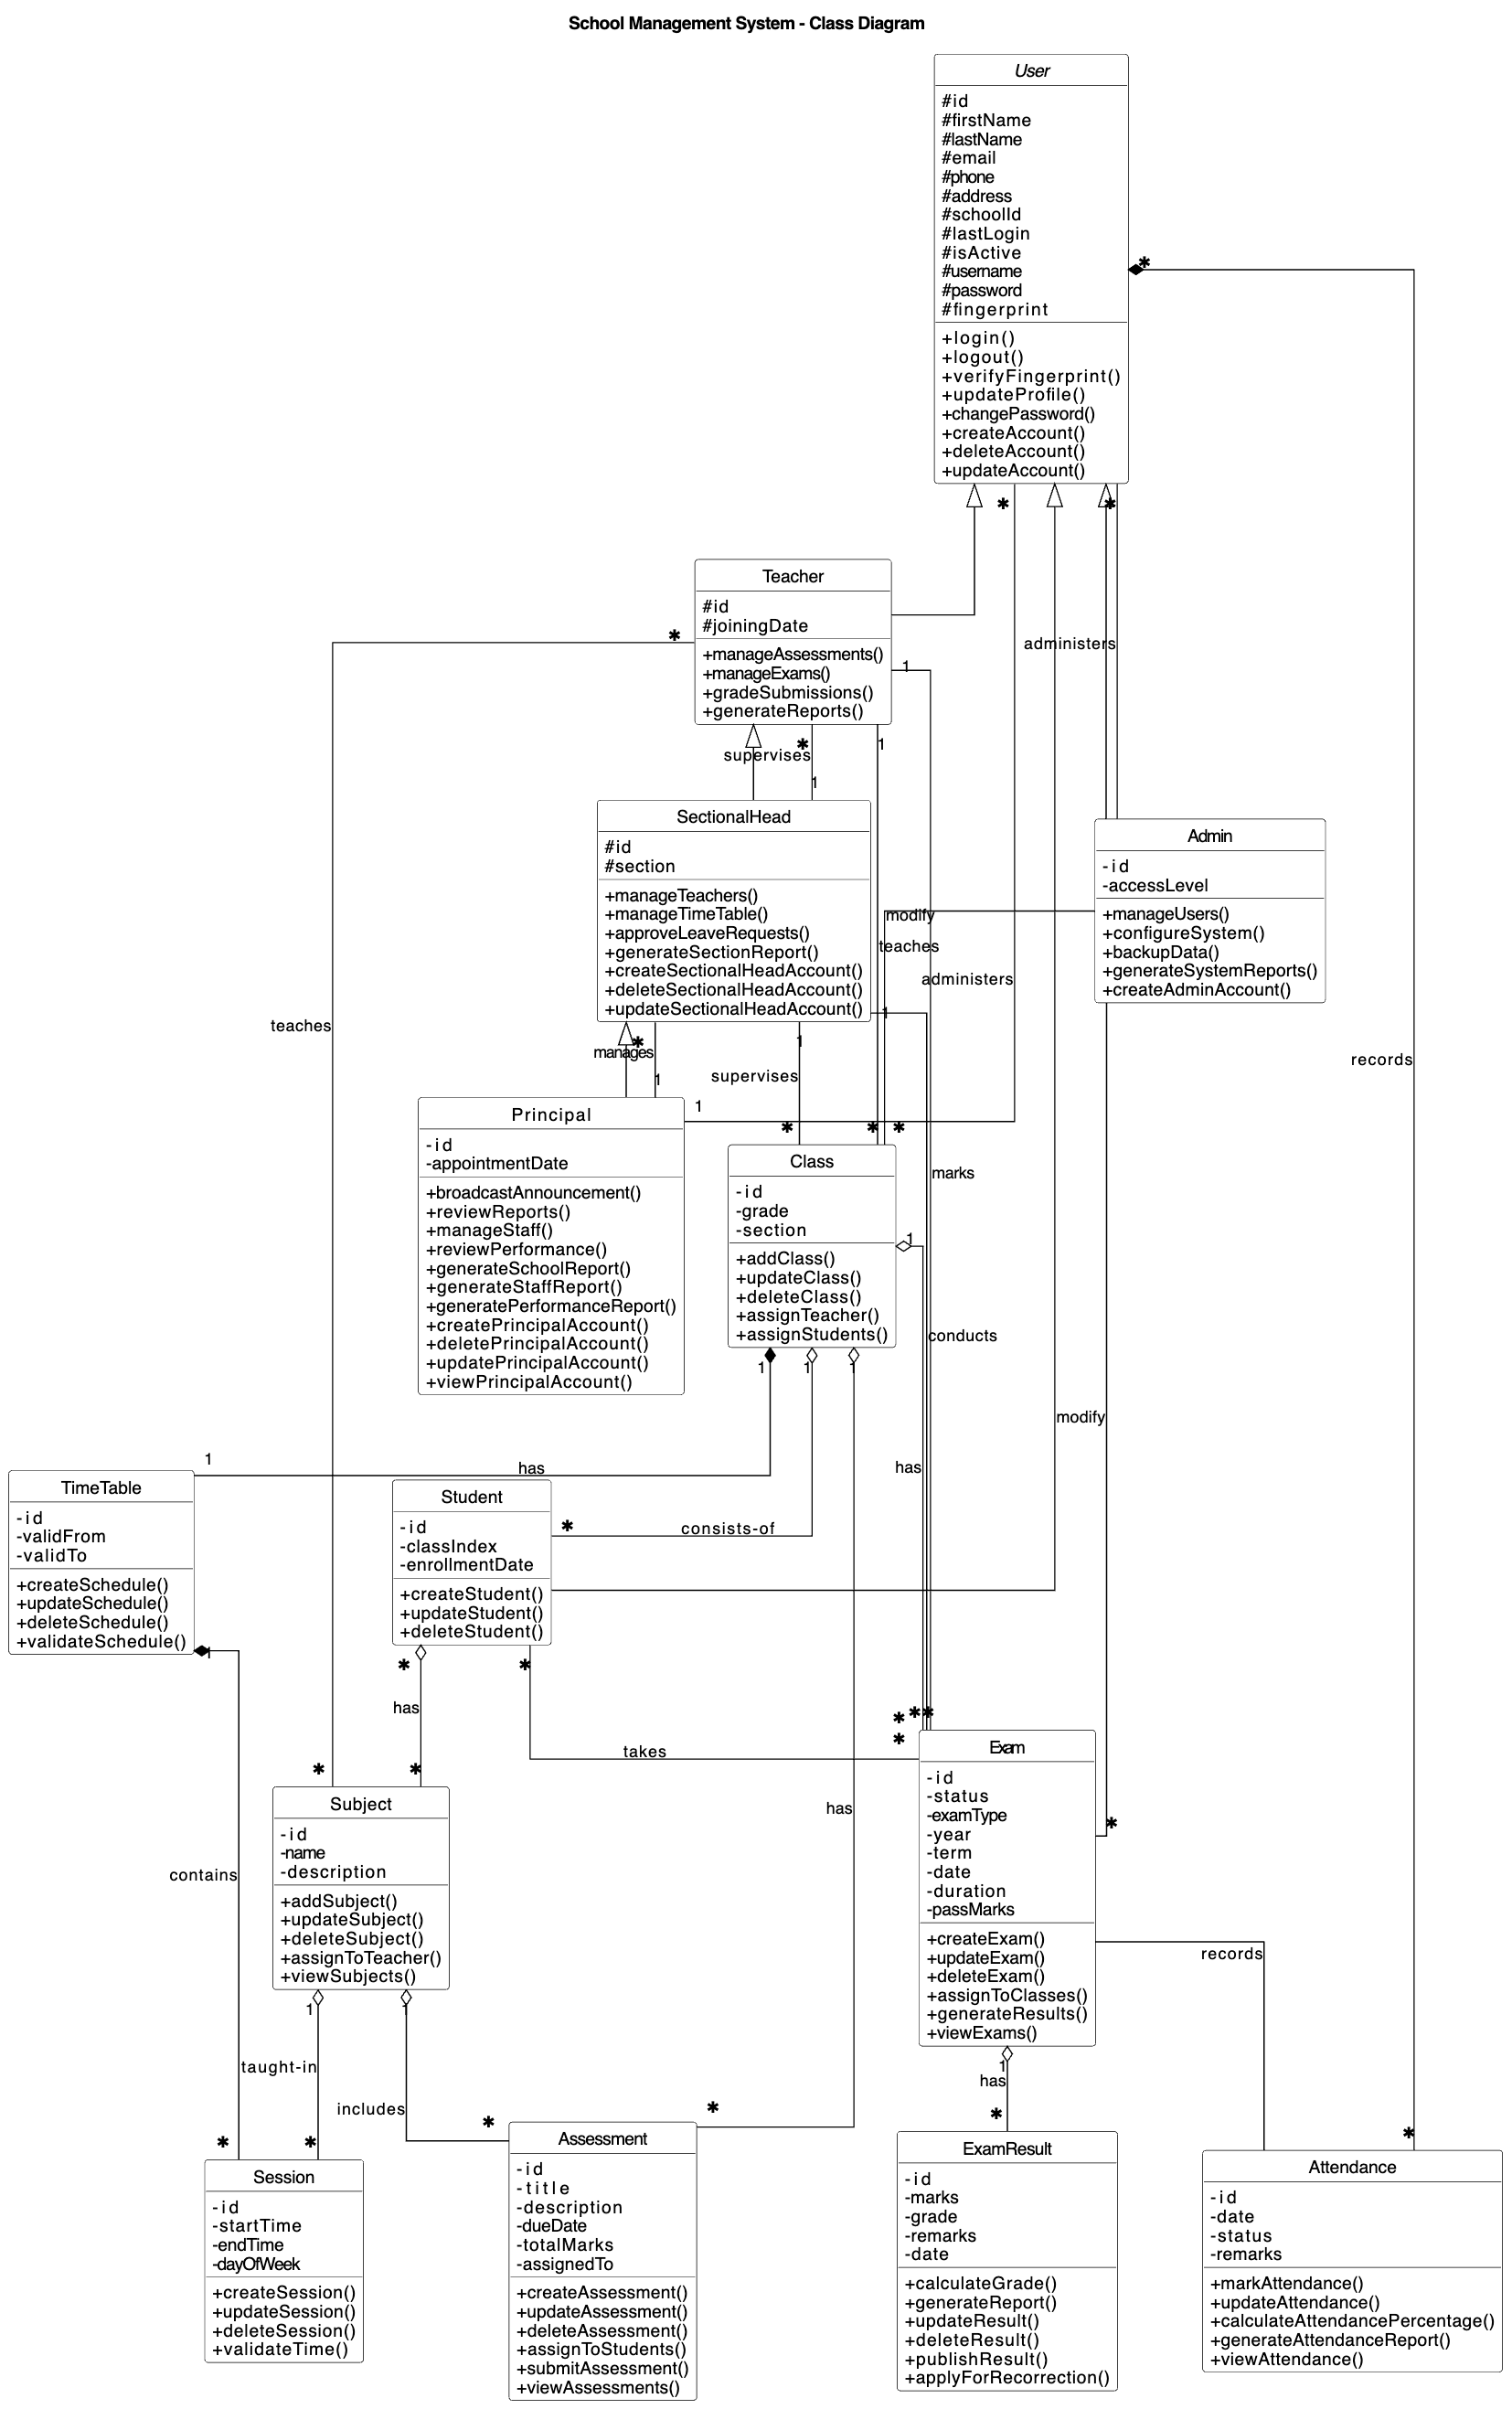
\includegraphics[width=1\textwidth]{class-diagram.png}
    \caption{Class Diagram}
    \label{fig:class-diagram}
\end{figure}

\subsection{Use Case Diagram}
\begin{figure}[htbp]
    \centering
    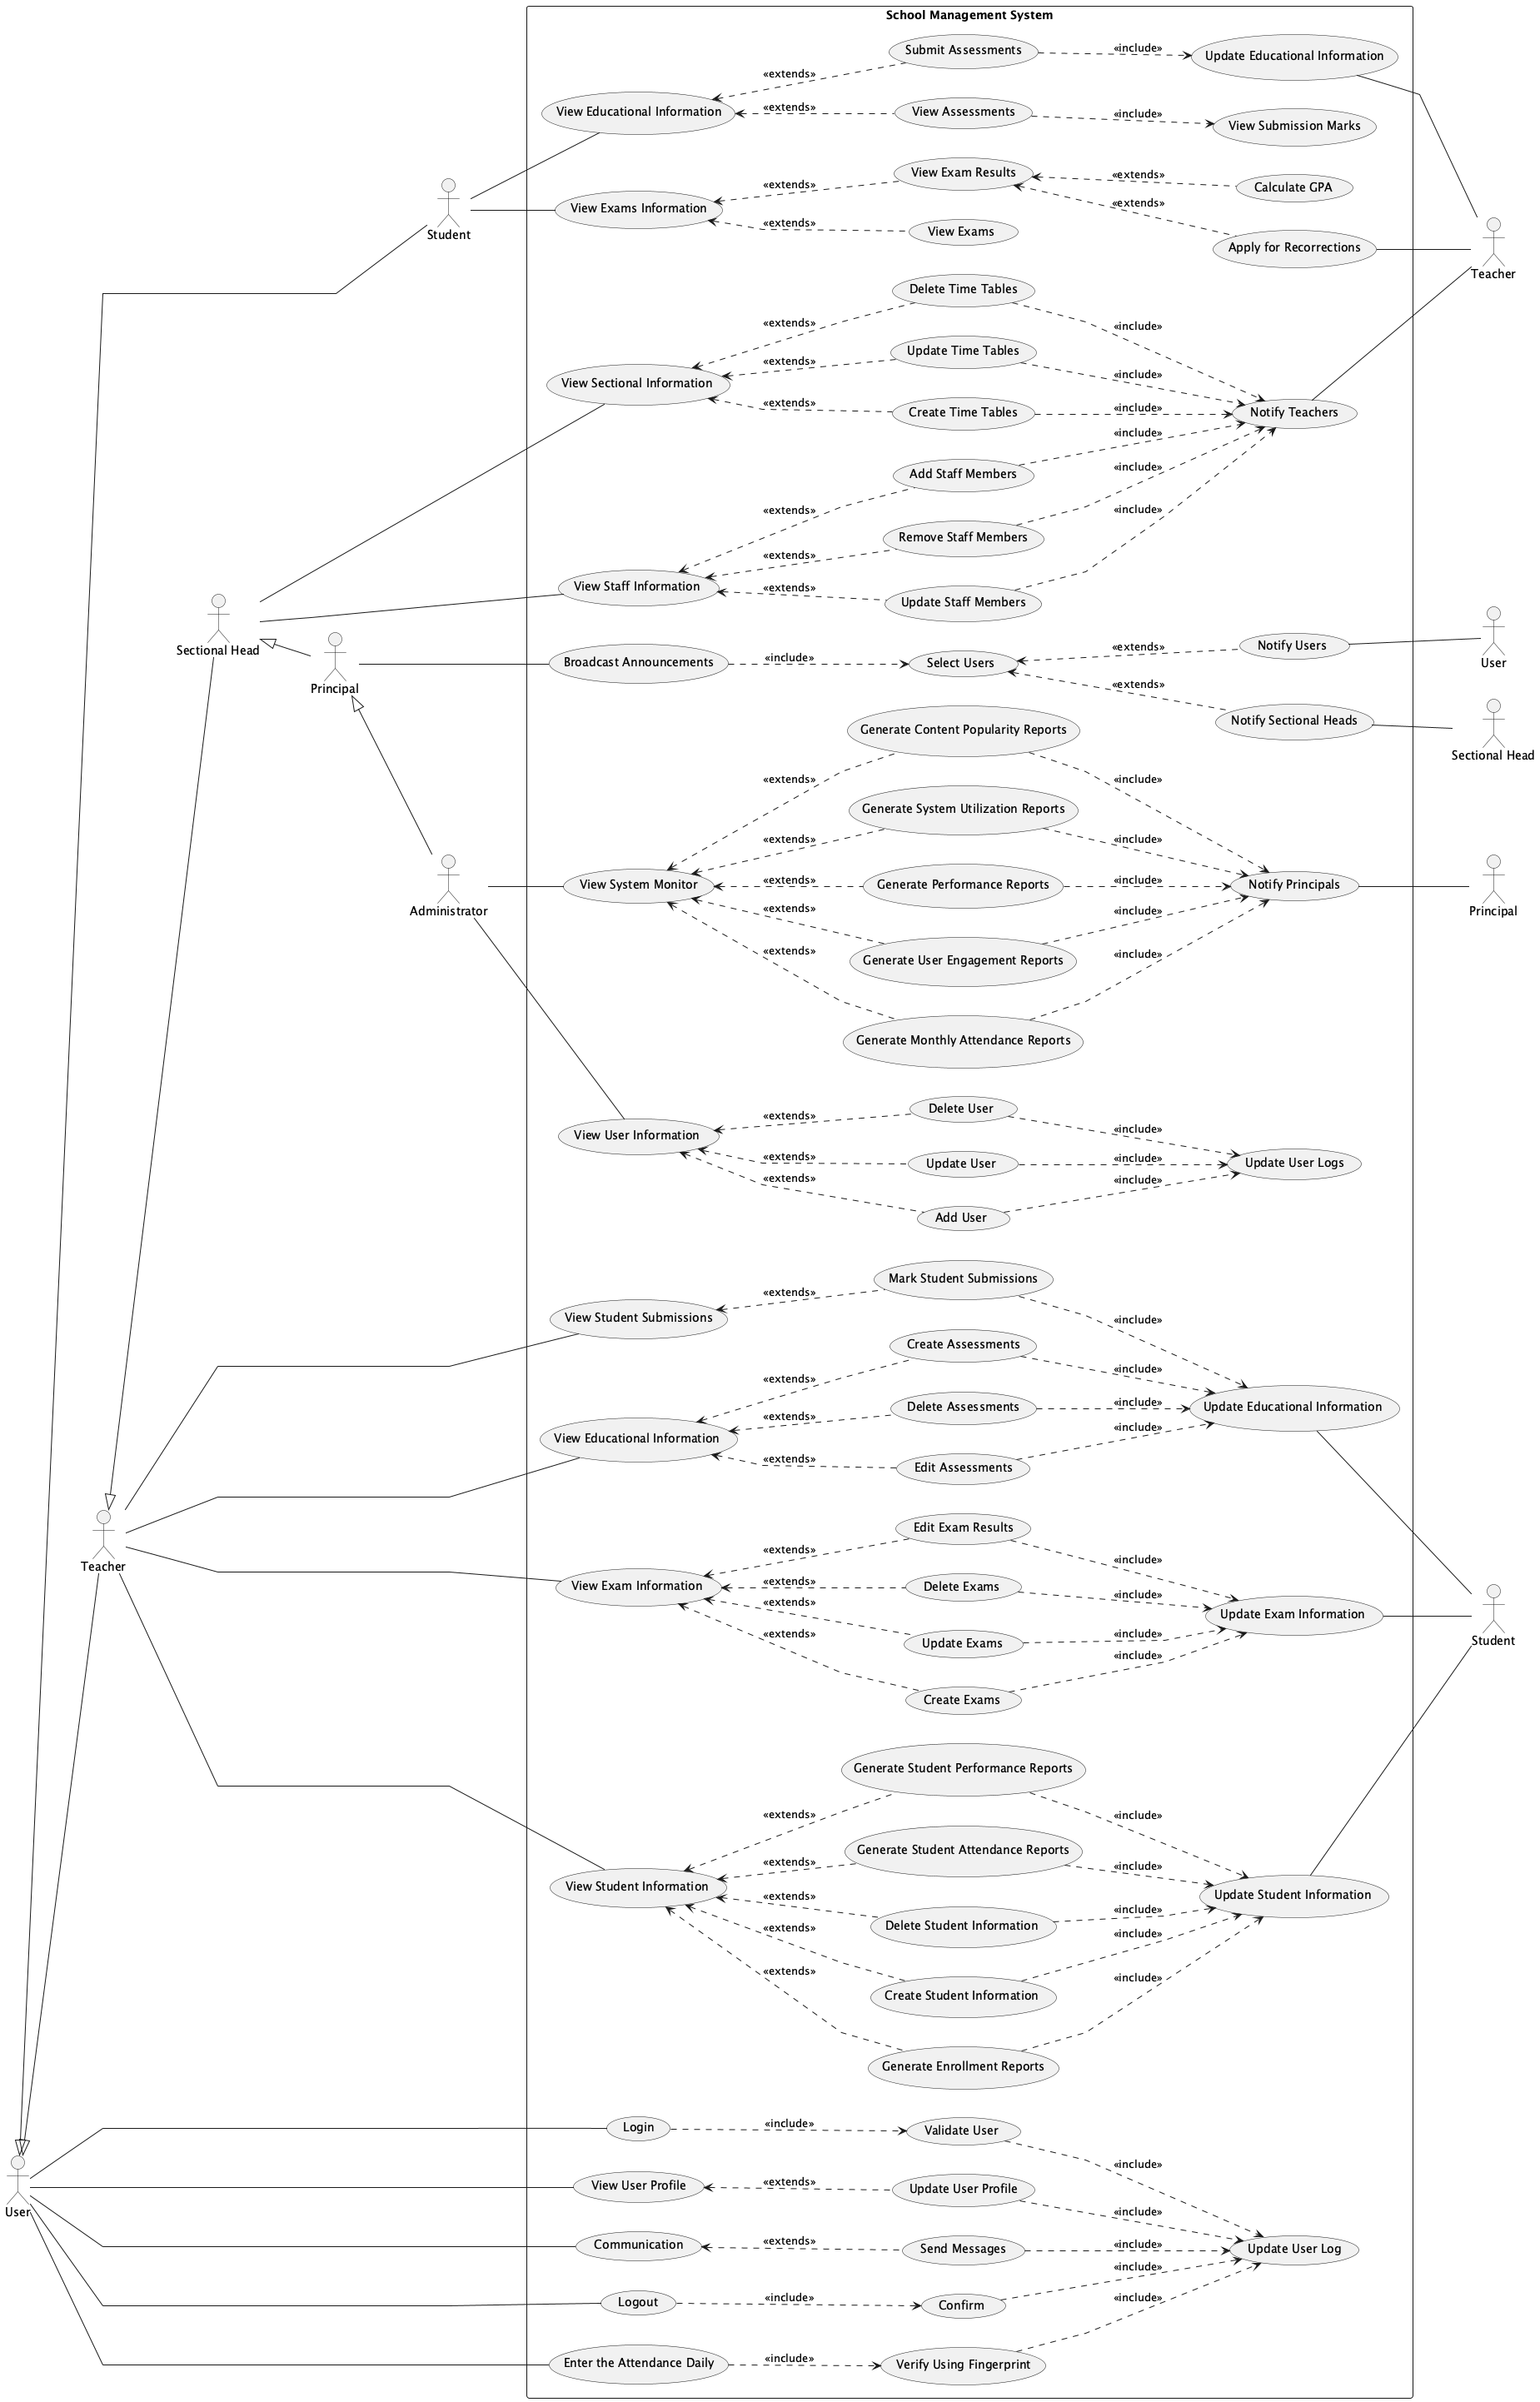
\includegraphics[width=1\textwidth]{use-case-diagram.png}
    \caption{Use Case Diagram}
    \label{fig:use-case-diagram}
\end{figure}

\chapter{User Interface Design}
\section{Login Page}
\begin{figure}[htbp]
    \centering
    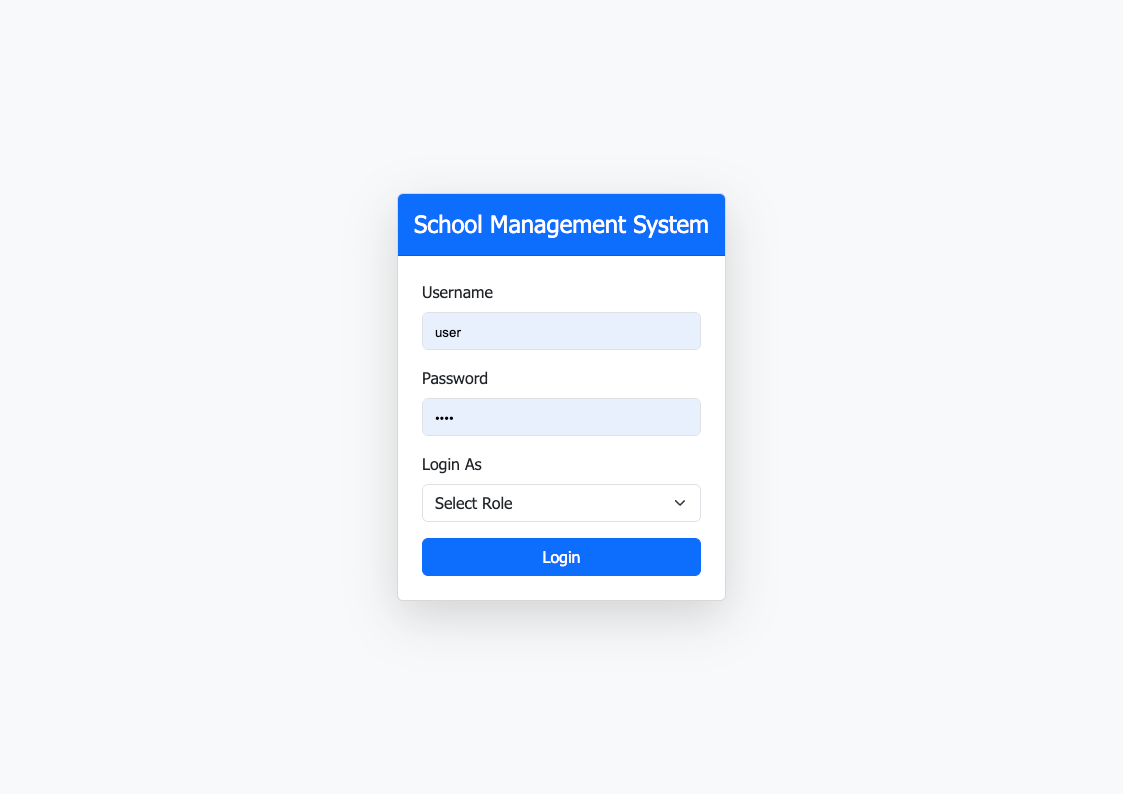
\includegraphics[width=0.8\textwidth]{login-page.png}
    \caption{Login Page}
    \label{fig:login-page}
\end{figure}

\section{Admin Dashboard}
\begin{figure}[htbp]
    \centering
    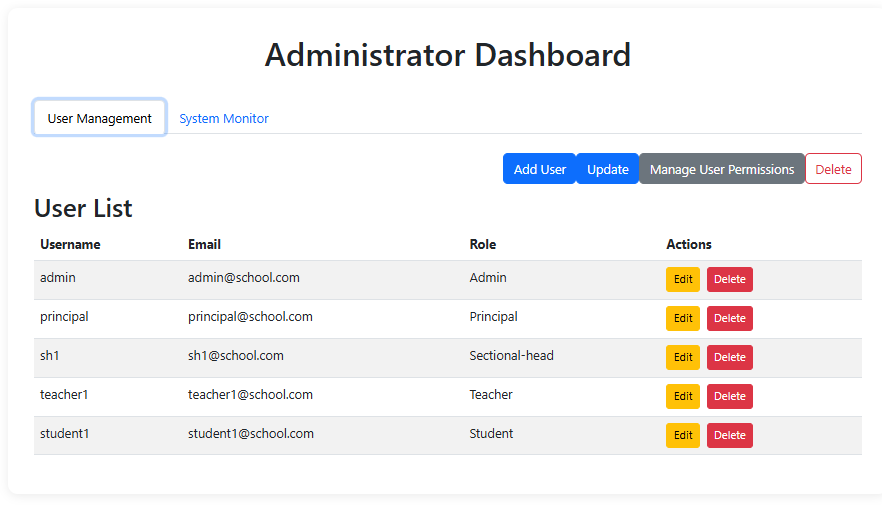
\includegraphics[width=1\textwidth]{admin-dashboard-page.png}
    \caption{Admin Dashboard Page}
    \label{fig:admin-dashboard-page}
\end{figure}

\chapter{Sequence Diagrams}
\section{Admin User Management}
\begin{figure}[htbp]
    \centering
    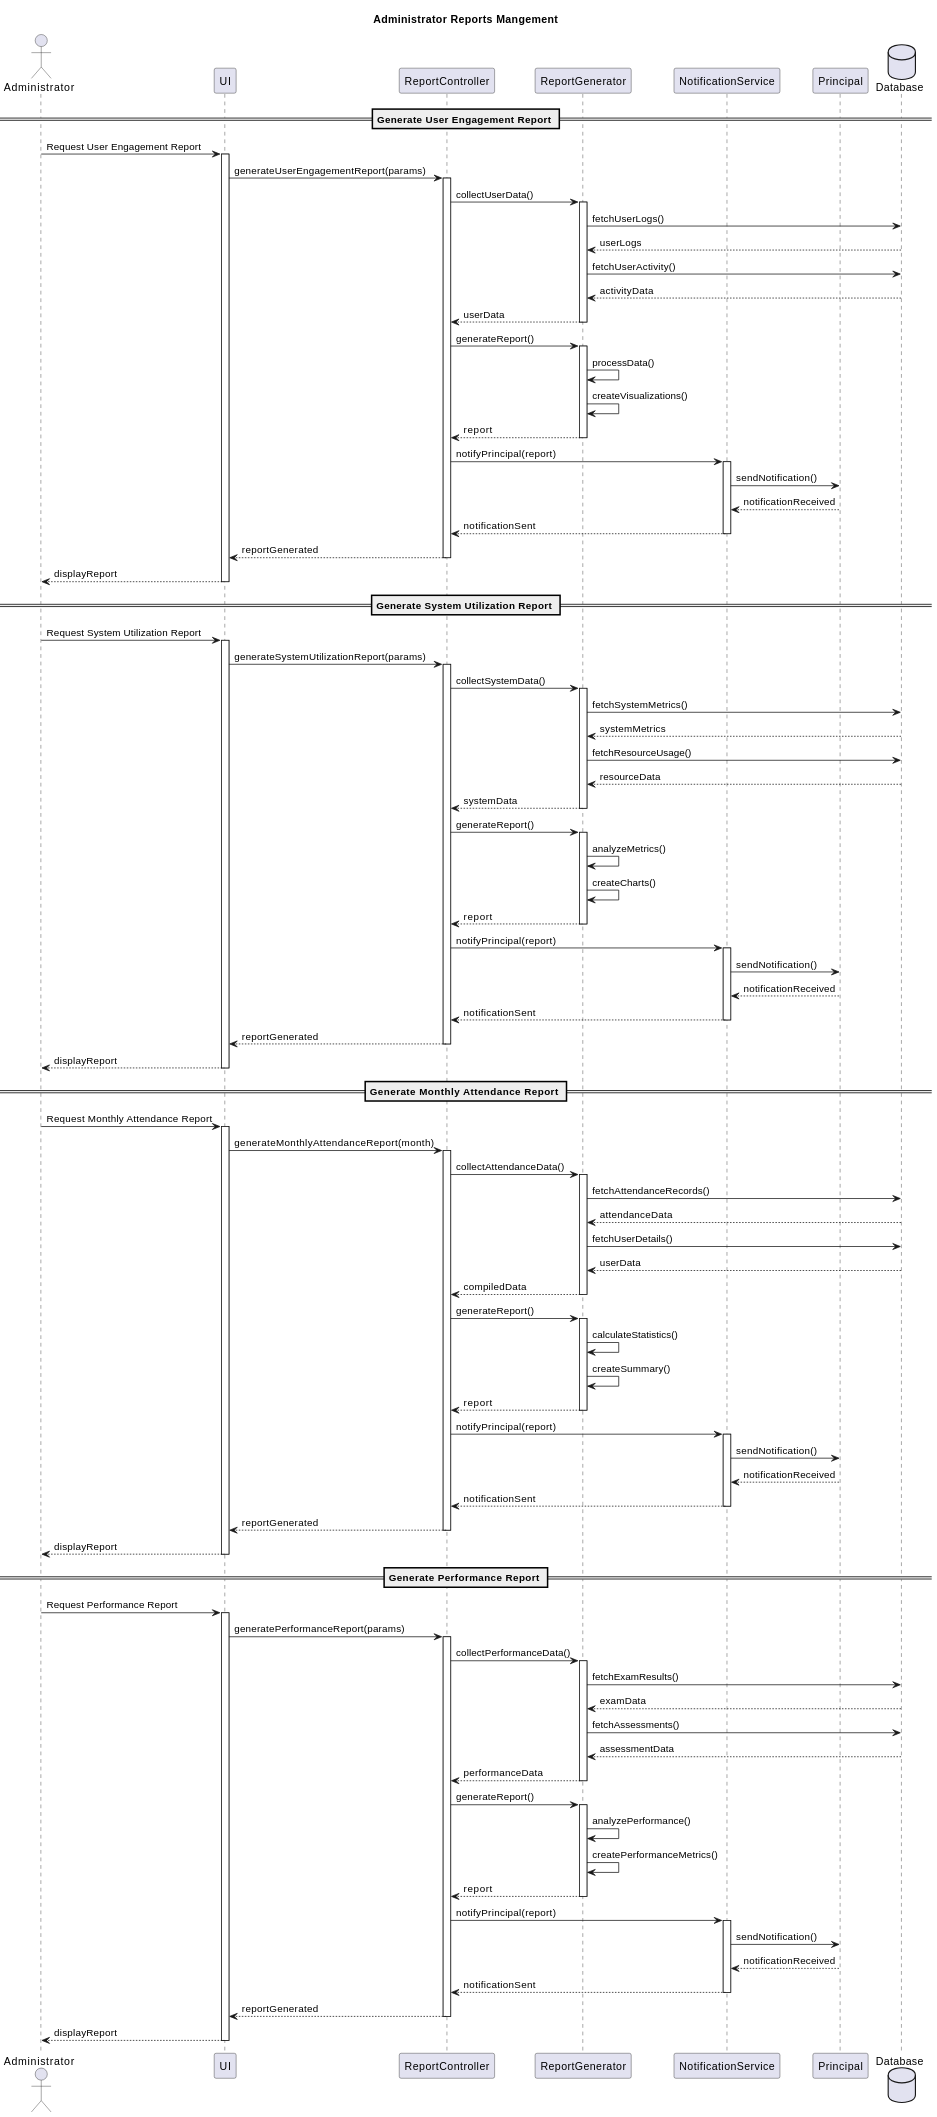
\includegraphics[width=0.8\textwidth]{admin-user-managment-sequence.png}
    \caption{Admin User Management Sequence}
    \label{fig:admin-user-managment-sequence}
\end{figure}

\section{Administrator Report Management}
\begin{figure}[htbp]
    \centering
    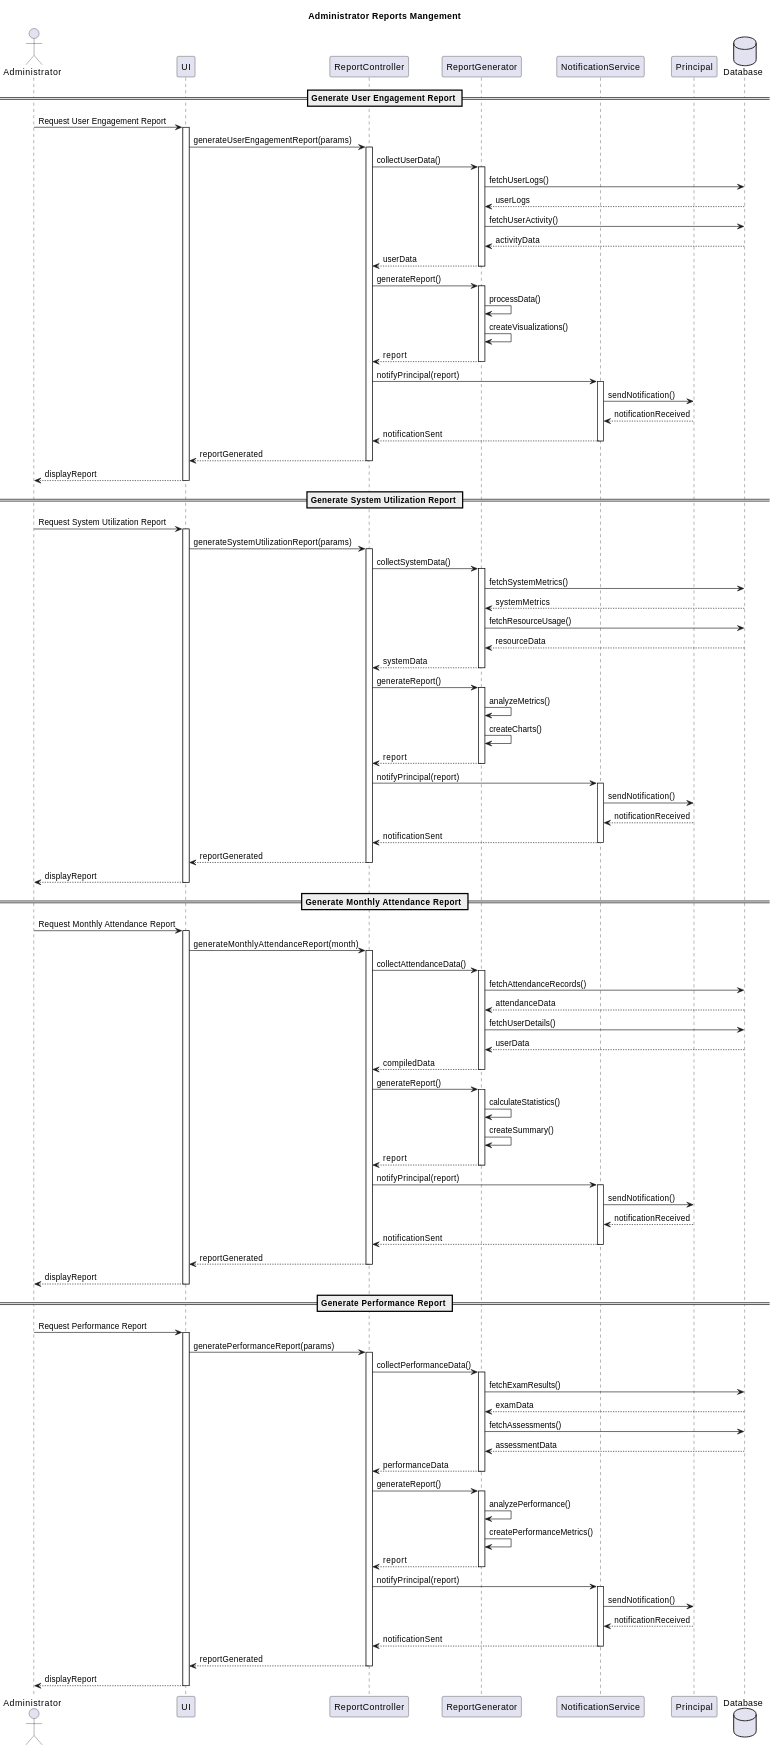
\includegraphics[width=1\textwidth]{administrator-report-management-sequence.png}
    \caption{Administrator Report Management Sequence}
    \label{fig:administrator-report-management-sequence}
\end{figure}

\section{Assessment Sequence}
\begin{figure}[htbp]
    \centering
    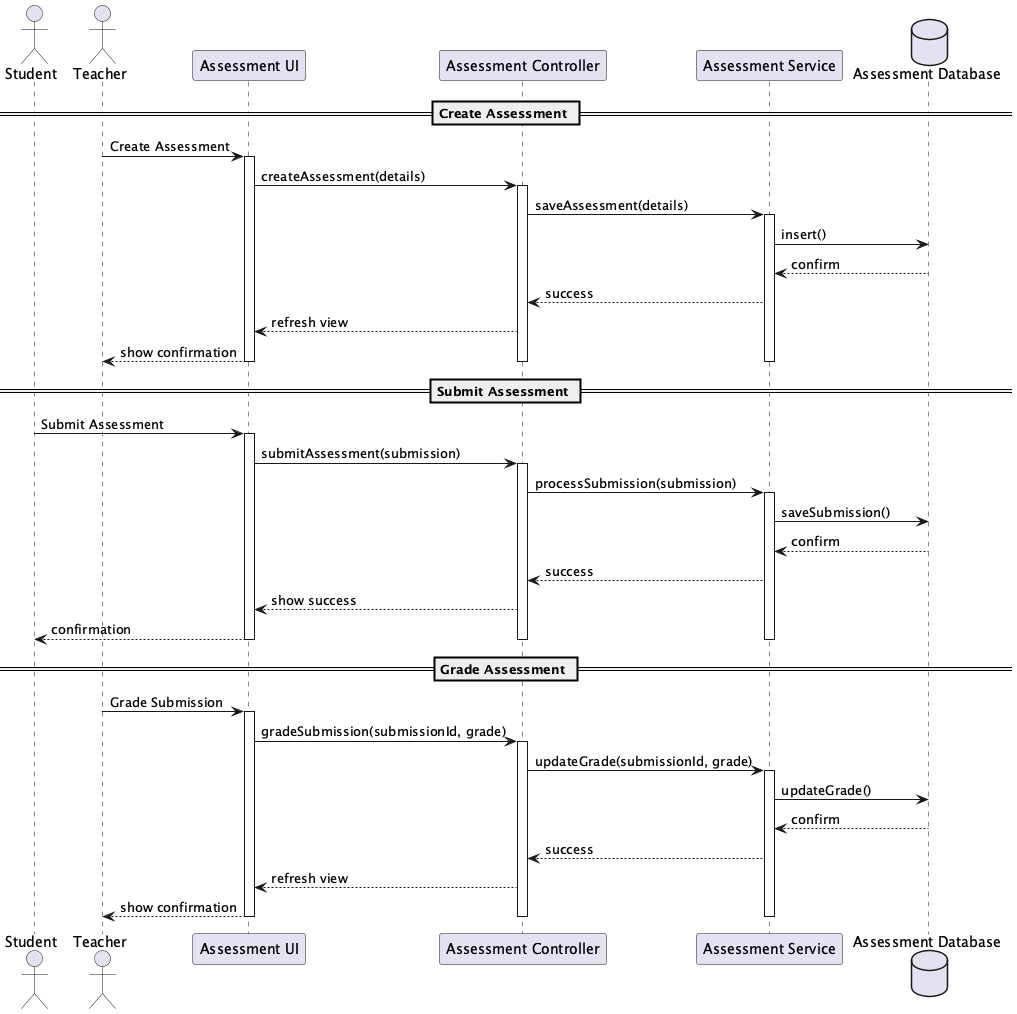
\includegraphics[width=1\textwidth]{assessment-sequence.png}
    \caption{Assessment Sequence}
    \label{fig:assessment-sequence}
\end{figure}

\section{Attendance Management Sequence}
\begin{figure}[htbp]
    \centering
    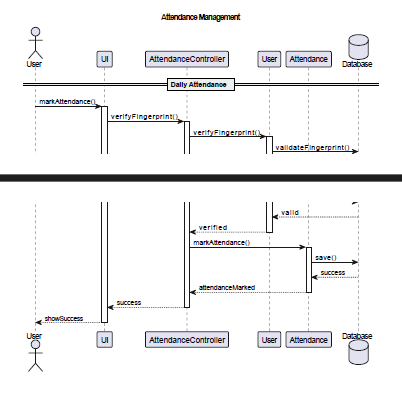
\includegraphics[width=1\textwidth]{attendance-management-sequence.png}
    \caption{Attendance Management Sequence}
    \label{fig:attendance-management-sequence}
\end{figure}

\section{Attendance Sequence}
\begin{figure}[htbp]
    \centering
    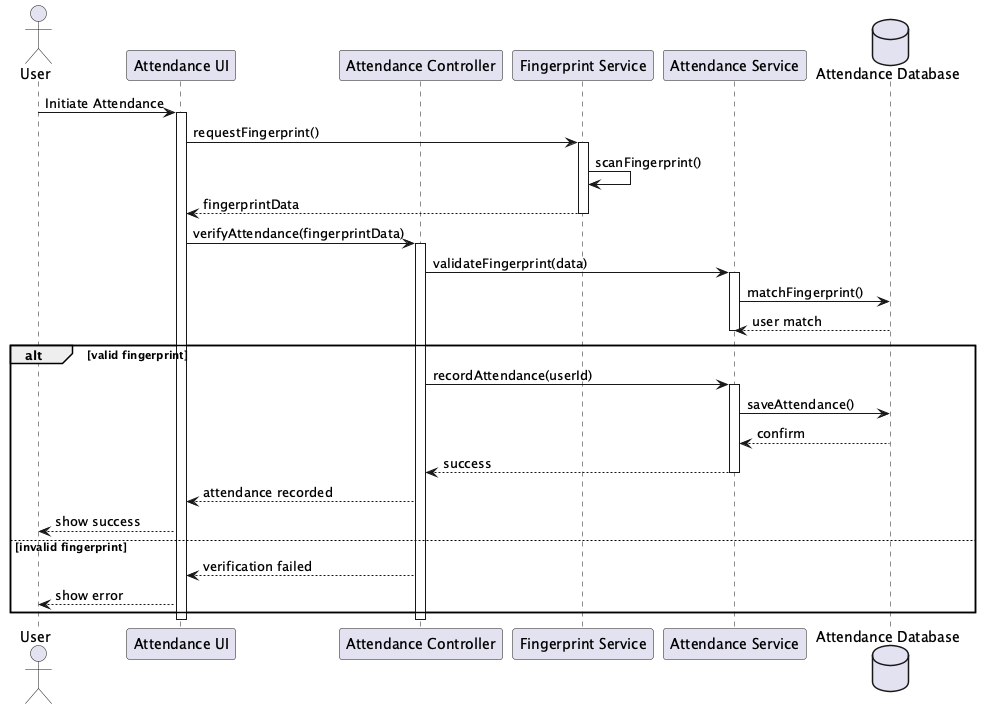
\includegraphics[width=1\textwidth]{attendance-sequence.png}
    \caption{Attendance Sequence}
    \label{fig:attendance-sequence}
\end{figure}

\section{Authentication Flow Sequence}
\begin{figure}[htbp]
    \centering
    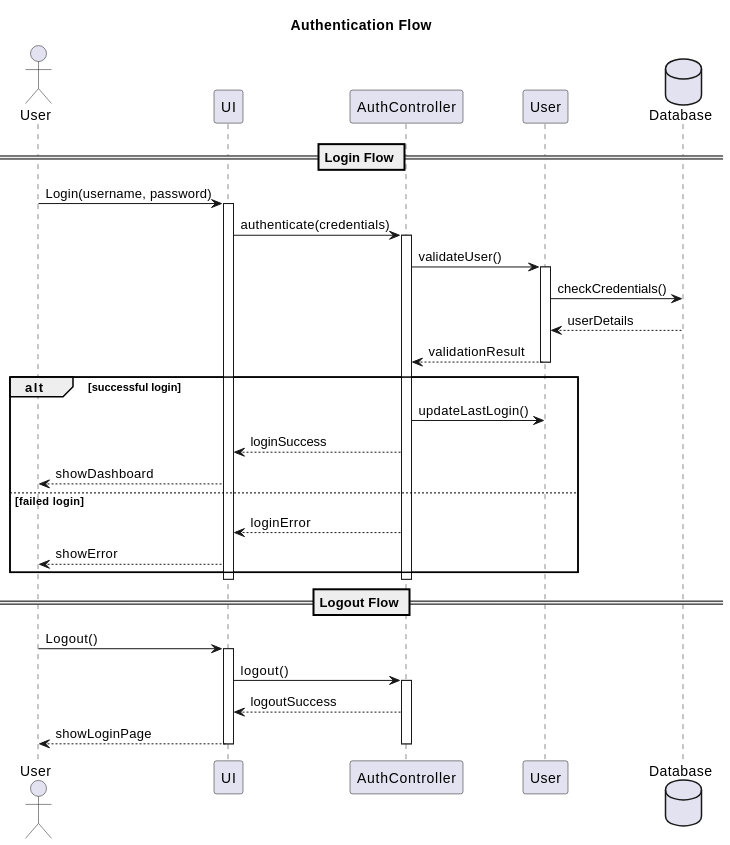
\includegraphics[width=1\textwidth]{authentication-flow-sequence.png}
    \caption{Authentication Flow Sequence}
    \label{fig:authentication-flow-sequence}
\end{figure}

\section{Authentication Sequence}
\begin{figure}[htbp]
    \centering
    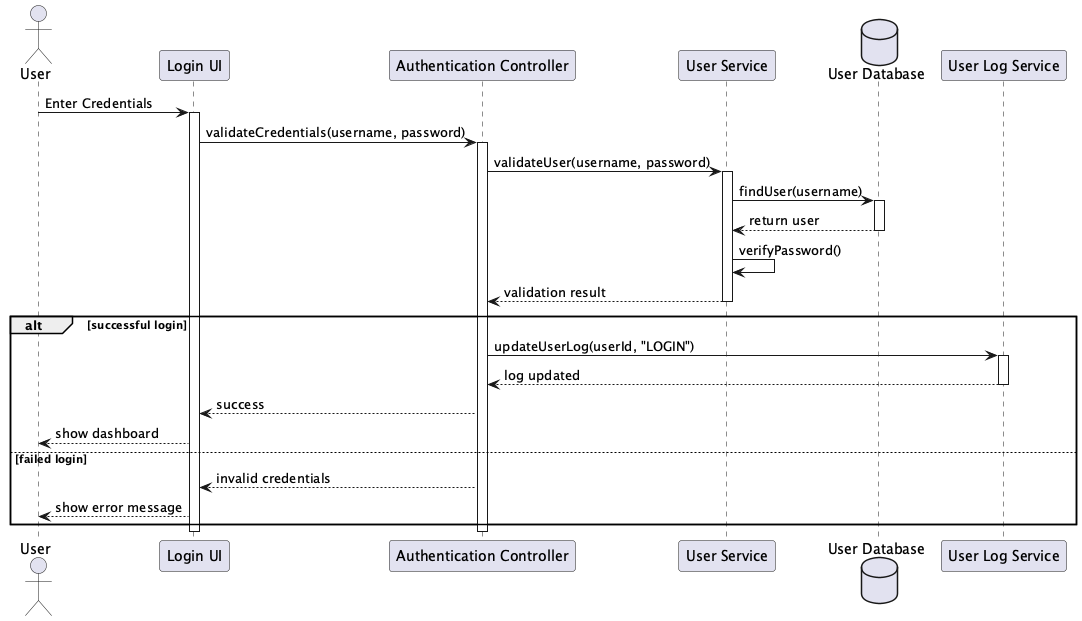
\includegraphics[width=1\textwidth]{authentication-sequence.png}
    \caption{Authentication Sequence}
    \label{fig:authentication-sequence}
\end{figure}

\section{Communication Flow Sequence}
\begin{figure}[htbp]
    \centering
    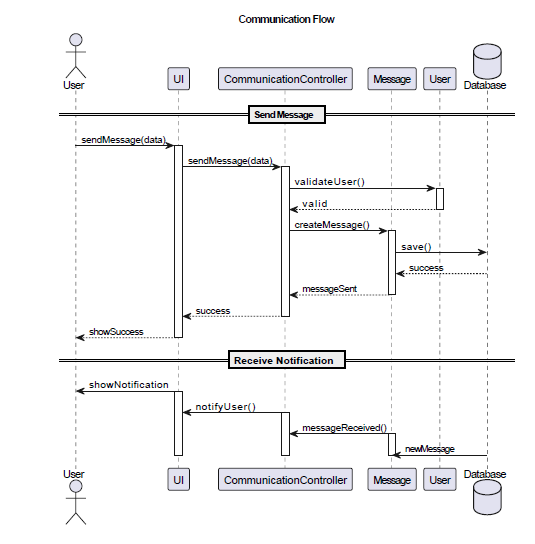
\includegraphics[width=1\textwidth]{communication-flow-sequence.png}
    \caption{Communication Flow Sequence}
    \label{fig:communication-flow-sequence}
\end{figure}

\section{Exam Management Sequence}
\begin{figure}[htbp]
    \centering
    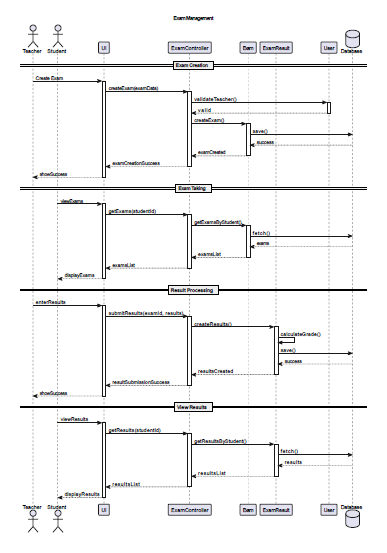
\includegraphics[width=1\textwidth]{exam-management-sequence.png}
    \caption{Exam Management Sequence}
    \label{fig:exam-management-sequence}
\end{figure}

\section{Exam Sequence}
\begin{figure}[htbp]
    \centering
    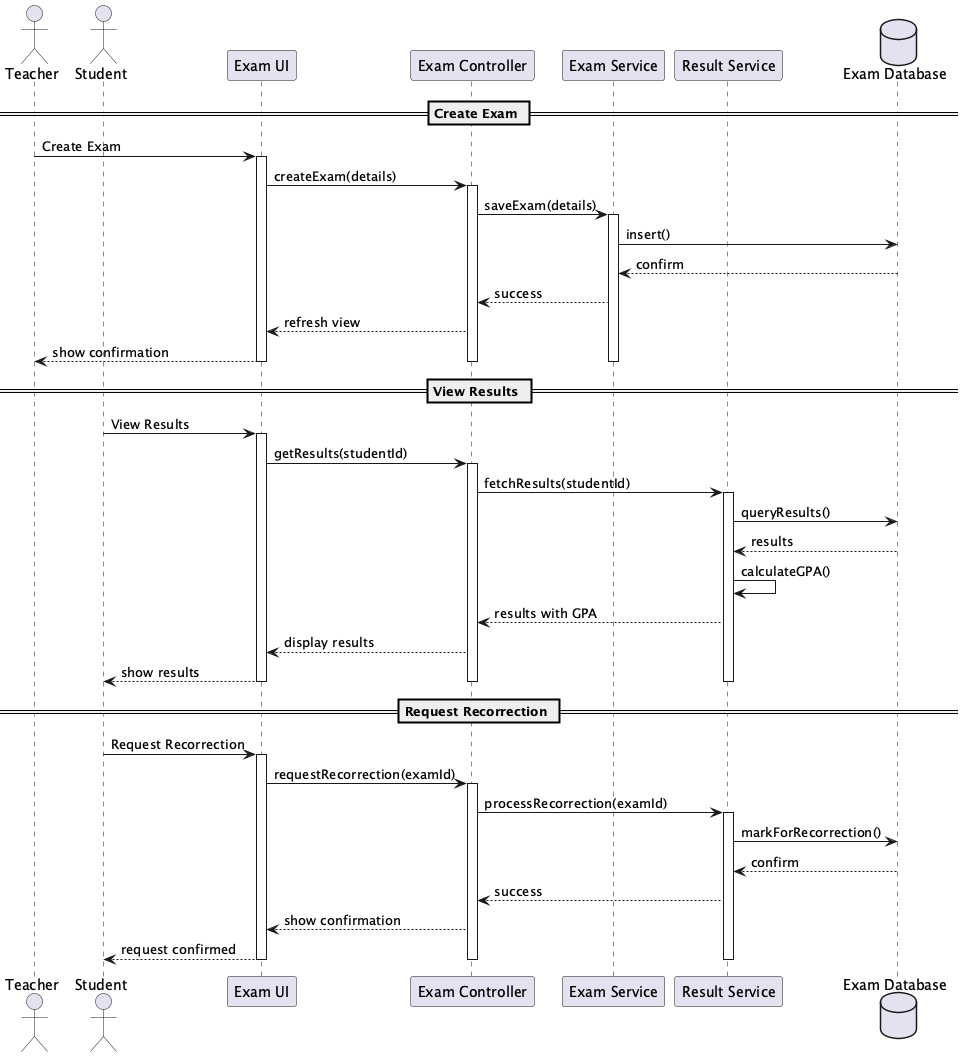
\includegraphics[width=1\textwidth]{exam-sequence.png}
    \caption{Exam Sequence}
    \label{fig:exam-sequence}
\end{figure}

\section{Generate Monthly Report dministrator Sequence}
\begin{figure}[htbp]
    \centering
    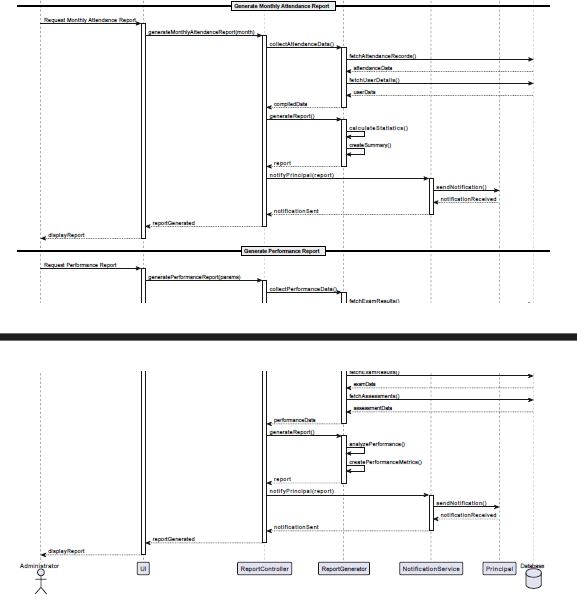
\includegraphics[width=1\textwidth]{generate-monthly-report-dministrator-sequence.png}
    \caption{Generate Monthly Report dministrator Sequence}
    \label{fig:generate-monthly-report-dministrator-sequence}
\end{figure}

\section{Principal Broadcast Sequence}
\begin{figure}[htbp]
    \centering
    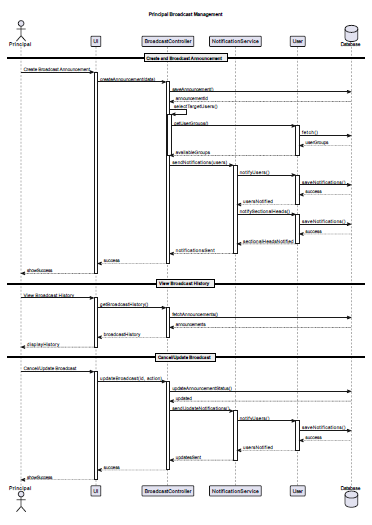
\includegraphics[width=1\textwidth]{principal-broadcast-sequence.png}
    \caption{Principal Broadcast Sequence}
    \label{fig:principal-broadcast-sequence}
\end{figure}

\section{Sectional Head Staff Management Sequence}
\begin{figure}[htbp]
    \centering
    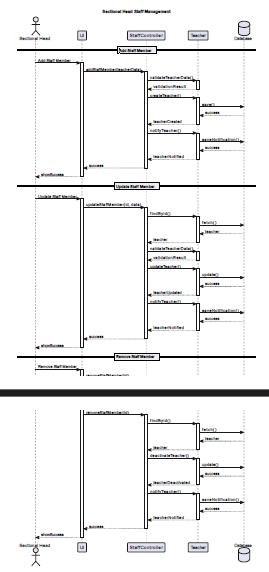
\includegraphics[width=0.7\textwidth]{sectional-head-staff-management-sequence.png}
    \caption{Sectional Head Staff Management Sequence}
    \label{fig:sectional-head-staff-management-sequence}
\end{figure}

\section{Student Assesment Management Sequence}
\begin{figure}[htbp]
    \centering
    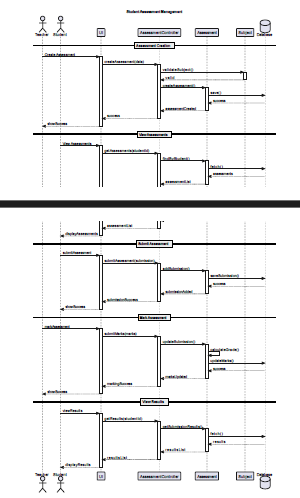
\includegraphics[width=0.9\textwidth]{student-assesment-management-sequence.png}
    \caption{Student Assesment Management Sequence}
    \label{fig:student-assesment-management-sequence}
\end{figure}

%%%%%%%%%%%%%%%%%%%%%%%%%%%%%%%%%%%%%%%%%%%%%%%%%%%%%%%%%%%%%%
% Chapter 5: Conclusion
%%%%%%%%%%%%%%%%%%%%%%%%%%%%%%%%%%%%%%%%%%%%%%%%%%%%%%%%%%%%%%
\chapter{Conclusion}
The School Management System represents a significant step forward in educational institution management. By addressing current system limitations and incorporating modern technology, the system promises to:
\begin{itemize}
    \item Improve administrative efficiency
    \item Support data-driven decision making
\end{itemize}

The modular design ensures future scalability and adaptability to changing educational needs.

%%%%%%%%%%%%%%%%%%%%%%%%%%%%%%%%%%%%%%%%%%%%%%%%%%%%%%%%%%%%%%
% References
%%%%%%%%%%%%%%%%%%%%%%%%%%%%%%%%%%%%%%%%%%%%%%%%%%%%%%%%%%%%%%
\newpage
\begin{thebibliography}{9}
    \bibitem{ref1} Diploma in Software Engineering Project Guidelines, NIBM
    % Add more references as needed
\end{thebibliography}

%%%%%%%%%%%%%%%%%%%%%%%%%%%%%%%%%%%%%%%%%%%%%%%%%%%%%%%%%%%%%%
% Appendices
%%%%%%%%%%%%%%%%%%%%%%%%%%%%%%%%%%%%%%%%%%%%%%%%%%%%%%%%%%%%%%
\appendix
\chapter{Appendices}
\section{Project Schedule}
% Include project timeline table or Gantt chart here

\section{Questionnaires and Interview Questions}
% Placeholder for data collection instruments

\section{Meeting Minutes and Log Sheets}
% Placeholder for meeting documentation

\section{Reviewed Documents}
% Placeholder for reviewed documents

\section{Permission Letter}

\begin{figure}[htbp]
    \centering
    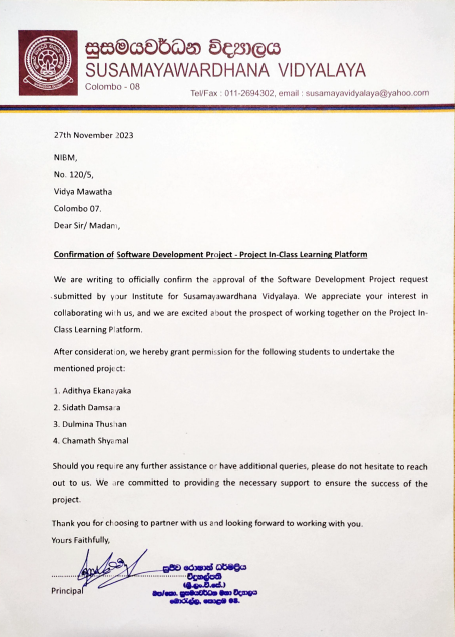
\includegraphics[width=0.8\textwidth]{school-permission-lettter.png}
    \caption{School Permission Letter}
    \label{fig:permission-letter}
\end{figure}

%%%%%%%%%%%%%%%%%%%%%%%%%%%%%%%%%%%%%%%%%%%%%%%%%%%%%%%%%%%%%%
% End of Document
%%%%%%%%%%%%%%%%%%%%%%%%%%%%%%%%%%%%%%%%%%%%%%%%%%%%%%%%%%%%%%
\end{document}
